%% This is file `ycviu-template.tex',
%% 
%% Copyright 2013 Elsevier Ltd
%% 
%% This file is part of the 'Elsarticle Bundle'.
%% ---------------------------------------------
%% 
%% It may be distributed under the conditions of the LaTeX Project Public
%% License, either version 1.2 of this license or (at your option) any
%% later version.  The latest version of this license is in
%%    http://www.latex-project.org/lppl.txt
%% and version 1.2 or later is part of all distributions of LaTeX
%% version 1999/12/01 or later.
%% 
%% The list of all files belonging to the 'Elsarticle Bundle' is
%% given in the file `manifest.txt'.
%% 
%% Template article for Elsevier's document class `elsarticle'
%% with harvard style bibliographic references
%%
%% $Id: ycviu-template-with-authorship.tex 69 2016-07-29 10:15:25Z aptara $
%%
%% This template has no review option
%% 
%% Use the options `twocolumn,final' to obtain the final layout
\documentclass[times,referee,twocolumn,final,authoryear]{elsarticle}

%% Stylefile to load YCVIU template
\usepackage{ycviu}
\usepackage{framed,multirow}

%% The amssymb package provides various useful mathematical symbols
\usepackage{amssymb}
\usepackage{latexsym}
\usepackage{amsmath}
\usepackage{dsfont}
\usepackage{amsfonts}
\usepackage{bigdelim}
%\usepackage[section]{placeins}
\usepackage{graphicx}
\usepackage{caption}
\usepackage{subcaption}

% Following three lines are needed for this document.
% If you are not loading colors or url, then these are
% not required.
\usepackage{url}
\usepackage{xcolor}
\definecolor{newcolor}{rgb}{.8,.349,.1}

\journal{Computer Vision and Image Understanding}

\begin{document}

\setcounter{page}{1}

\begin{frontmatter}

\title{Attention mechanism for collision-free grasp detection from 3D point clouds}

\author[1]{Dinh-Cuong \snm{Hoang}\corref{cor1}} 
\cortext[cor1]{Corresponding author: 
  Tel.: +0-000-000-0000;  
  fax: +0-000-000-0000;}
\ead{hoangcuongbk80@gmail.com; cuonghd7@fe.edu.vn}
\author[1]{Bao-Long \snm{Tran}}
%\author[2]{Given-name \snm{Surname}}

\address[1]{ICT Department, FPT University, Hanoi, Vietnam}
%\address[2]{Affiliation 2, Address, City and Postal Code, Country}

\received{1 May 2013}
\finalform{10 May 2013}
\accepted{13 May 2013}
\availableonline{15 May 2013}
\communicated{S. Sarkar}

\begin{abstract}

Grasp detection is a challenging and important task in robotics and computer vision. Many existing methods require time-consuming multi-stage processing for sampling grasp candidates and evaluating the grasp quality. While several works proposed end-to-end models for 6-DOF grasp detection and achieved state-of-the-art results in benchmarks. However, most of these models treat all points in a scene equally without focusing on the more relevant regions, which greatly harms the speed and accuracy. Inspired by the success of the attention mechanism in various computer vision tasks, this work discovers the power of the attention mechanism to boost the performance of grasp detection from 3D point clouds. To achieve this, taking the recent  VoteGrasp (\textcolor{cyan}{\cite{hoang2022context}}) as a basic pipeline, we integrate different attention modules into the end-to-end grasp detection network and provides insights into the potential of these modules.

\end{abstract}

\begin{keyword}
\MSC 41A05\sep 41A10\sep 65D05\sep 65D17
\KWD Keyword1\sep Keyword2\sep Keyword3

 MSC codes here, in the form: \MSC code \sep code
%% or \MSC[2008] code \sep code (2000 is the default)
\end{keyword}

\end{frontmatter}

%\linenumbers

%% main text

%%%%%%%%%%%%%%%%%%%%%%%%%%%%%%%%%%%%%%%%%%%%%%%%%%%%%%%%%%%%%%%%%%%%%%

\section{Introduction}
\label{sec:intro}
Conventional methods for grasp detection consider accurate estimation of 6D pose as a fundamental. These approaches typically consist in recovering correspondences between CAD models and object point clouds to register grasps from pre-computed database (\textcolor{cyan}{\cite{munoz2016fast}}, \textcolor{cyan}{\cite{zeng2017multi}}). The grasps are previously calculated for CAD models and then to be regressed to determine high-quality one for objects (\textcolor{cyan}{\cite{bohg2013data}}). Some approaches obtain 6D pose estimation by employing algorithms such as iterative closest point (\textcolor{cyan}{\cite{besl1992method}}) to align models to point clouds or exploiting local descriptors such as SIFT key points (\textcolor{cyan}{\cite{dias2014sift}}) for 3D matching. Whereas, recent approaches leverage the advance of deep learning technique to design end-to-end models for predicting 6DoF rotation and translation vector in 3D space (\textcolor{cyan}{\cite{wu20196d}}, \textcolor{cyan}{\cite{wang2019densefusion}}). In general, however, the heavy dependencies of these methods on 3D CAD models, which might be not always available for all objects or might require intensive labor in the pre-scanning process, restricts their ability to be widely applied in all scenarios.

This motivated alternative approaches that directly detect grasps from sensor data thanks to CNN without estimating object pose. In other words, instead of registering point clouds to a pre-computed dataset and indexing grasps, these methods learn to identify a set of candidates and the probability of success of grasps. In recent works, (\textcolor{cyan}{\cite{mahler2017dex}}, \textcolor{cyan}{\cite{mahler2018dex}}) apply deep CNNs to find features, while others (\textcolor{cyan}{\cite{redmon2015real}}, \textcolor{cyan}{\cite{lenz2015deep}}) develop end-to-end learning for estimating possible grasps. The results of learning-based approaches allow to grasp pre-known objects, which might be partially occluded, an unknown pose as well as fully novel objects.

Grasp detection area differs from object detection and pose estimation due to it requires both determining grasp candidates and maximining the probability of success of grasps. To generate quality candidates, which are understood as reasoning parts of objects for the gripper to appropriately operate, it seems to be inadequate to consider only 2D or 2.5D local features of objects since focusing on visual similarities might lead to failure in some cases, especially in occlusion context and texture-less objects. Therefore, a few approaches (\textcolor{cyan}{\cite{ten2017grasp}}, \textcolor{cyan}{\cite{mousavian20196}}, \textcolor{cyan}{\cite{liang2019pointnetgpd}}, \textcolor{cyan}{\cite{fang2020graspnet}}) take 3D geometry analysis into account to robust the performance of predicting grasp by localizing grasp from 3D point sets.

On the other hand, achieving highly feasible grasps is a challenging problem that researchers have to cope with. The successful grasps are considered to be not involved with undesirable contacts with surroundings. This is hardly achievable because of measurement noise in acquiring data, occlusion environments, and cluttered scenarios. In attempt to deal with this problem, several methods intensively collect numerous grasp candidates, while others propose end-to-end models for 6-DOF grasp detection. These end-to-end approaches achieve state-of-the-art result in benchmarks thanks to employing backbone networks such as PoinNet++ (\textcolor{cyan}{\cite{qi2017pointnet++}}) to take advantage of local property. Although these strategies could gain high-grade grasping points, they find hard to avoid unexpected collisions. Solely considering regional information of each candidate without examining the spatial relationship of neighboring candidates appears to be insufficient for system to be fully aware of context. Thus, the contextual information is a prospective material to be succeed in accomplishing collision-free grasps.

Motivated by the above perspective, we introduce an effective end-to-end model for 6-DOF grasp detection. It accomplishes highly competitive grasp configurations in severe scenarios of occlusion when compared with others in benchmarks. This success is attributed to the essence of leveraging both a voting mechanism architecture (\textcolor{cyan}{\cite{qi2019deep}}) to elect candidates and a context learning module to encode the spatial relationship of neighboring candidates into feature vectors. Voting mechanism allows our model to widen our model's capability to beforehand unknown objects. Besides, fusing contextual spatial features into local features enables our method to enhance the performance in alleviating potential collision. The following highlights the main contributions of our work:

%%%%%%%%%%%%%%%%%%%%%%%%%%%%%%%%%%%%%%%%%%%%%%%
\begin{itemize}
	\item Our research proposes a new robust framework VoteGrasp combing voting mechanism and contextual learning module for 6-DOF grasp detection and achieves remarkable results while operating in severe scenes of occlusions. Besides, our proposal demonstrates its generalization capability to novel objects.
	\item We develop a context learning module that contributes the spatial dependency of objects in candidates’ vicinity to the feature vectors to learn collision-free grasps. 
	\item Experiments compare the results of attention modules to find out what is most robust and suitable to our model.
\end{itemize}
 
%
\section{Related work}
\label{sec:related_work}

\subsection{3D Point Cloud Based Grasp Detection}
Robotic grasping is conventionally involved in two related problems of perception and planning. The perceptual component aims to acquire the position and orientation of the object to be grasped. The planning component considers how to evaluate a good manipulation. This primitive idea comes to 3D retrieval methods that retrieve segmented point clouds to 3D CAD models to estimate the object poses and then decide grasps from a pre-defined grasp dataset. As mentioned in previous sections, this old-fashioned approach is impractical in some cases due to the problem of the existence of all accurate CAD models. Furthermore, these methods could not detec grasps for novel objects outside of the dataset. 

To overcome these issues, machine learning-based approaches have been introduced to directly detect grasp from sensor data without estimating object pose with a conventional pipeline of grasp sampling process, extracting features of the grasps, and evaluating the quality of grasps. (\textcolor{cyan}{\cite{ten2017grasp}}) proposed grasp pose detection (GPD) algorithm from point clouds. Unlike (\textcolor{cyan}{\cite{herzog2012template}}), which necessarily segments the object from the background, this method first identifies a ROI that could include multiple objects or even background to find a grasp. The large set of grasp candidates is interested to be found in ROI with respect to two conditions of not being in collision with the point cloud and there being no contact between grippers and point cloud. Then, a four-layer CNN decides whether or not a candidate is a grasp for observed and occluded surfaces acquired from the depth sensor. As an extension of PGD idea, PointNetGPD (\textcolor{cyan}{\cite{liang2019pointnetgpd}}) replaces the CNN-based evaluation model with a new network based on architecture of PointNet (\textcolor{cyan}{\cite{qi2017pointnet}}). Taking advantage of PointNet architecture, this evaluation model can directly perform geometry analysis, which the original PGD idea lacks, from the 3D point cloud and therefore can detect more reliable grasps. However, these approaches could not provide good enough grasp assessments, they need exhaustively manual sampling grasps, which sometimes is hard to acquire when the raw point cloud is spare. This motivates the method (\textcolor{cyan}{\cite{mousavian20196}}) to introduce two network architectures for both sampling and evaluating grasps. Instead of manually sampling grasps, this one utilizes a variational auto-encoder (VAE) model to generate a diverse set of grasps as well as limit the number of failing grasps. Detecting grasps is important because not all grasps are kinematically feasible or collision-free for the manipulation of the robot. In terms of the evaluation model, this method not only classifies each grasp but also iteratively refines a significant portion of the rejected grasps to the successful ones. Nevertheless, all these approaches solely depend on the local visible parts of objects, which occasionally is imperfect due to the noisy depth value. Some methods sort to use high-quality depth sensors or utilize the multi-view technique (\textcolor{cyan}{\cite{ten2017grasp}}) to provide high-success rates of grasps.

The lack of geometric information about candidates’ surroundings and information about the scene mitigates the performance of the above methods. Perceiving this remaining issue, end-to-end methods (\textcolor{cyan}{\cite{fang2020graspnet}}, \textcolor{cyan}{\cite{ni2020pointnet++}}) take the whole point clouds as input and neglect the tradition pipeline of time-consuming grasp sampling process. They combine global data information to directly predict the poses and qualities of spatial grasps. Their PointNet++-based architectures allow them to immediately extract local spatial features from the raw data point clouds, while others such as (\textcolor{cyan}{\cite{choi2018learning}}) employs a three-dimensional deep learning neural network to deal with voxelized point clouds, which might be less precise in detail due to voxelization. Although considering whole point clouds, these approaches don’t take the relationship between objects into account and only focus on local representations of points. As a result, their performance in cluttered environments is unreliable. We address the remaining challenges by leveraging voting mechanisms combined with contextual information to ensure the generalization and reliability of grasps.

\subsection{Hough Voting in Object Detection}
The Hough Transform was originally informed to detect defined shapes in 2D space such as lines, circles, or eclipses (\textcolor{cyan}{\cite{hough1959machine}}, \textcolor{cyan}{\cite{hough1962method}}, \textcolor{cyan}{\cite{duda1972textordfeminineuse}}). This technique is limited to shapes characterized by a small number of parameters. The Generalized Hough Transform is then introduced to extend the application of the primitive algorithm to arbitrary shapes. It, therefore, is widely extended and applied to computer vision tasks including object detection (\textcolor{cyan}{\cite{gall2013class}}, \textcolor{cyan}{\cite{gall2011hough}}), motion detection (\textcolor{cyan}{\cite{gall2011hough}}, \textcolor{cyan}{\cite{kalviainen1996motion}}), medical imaging (\textcolor{cyan}{\cite{golemati2006comparison}}), and robot navigation (\textcolor{cyan}{\cite{iocchi2001probabilistic}}). In terms of 3D scenes, methods (\textcolor{cyan}{\cite{deng2018ppfnet}}, \textcolor{cyan}{\cite{rabbani2005efficient}}) utilizes the original Hough Transform formulation in a straightforward way to deal with 3D analytical shapes like spheres and cylinders. However, these methods cannot be applied to generic free-form objects, which are common in realistic applications.

More recently, several methods (\textcolor{cyan}{\cite{silberberg1984iterative}}, \textcolor{cyan}{\cite{tombari2010object}}) widen the use of Hough voting mechanisms to 3D object detection. (\textcolor{cyan}{\cite{tombari2010object}}) even proves the robustness of their approach in scenes with a significant degree of occlusions. They aim to deploy 3D features of interesting point, which is chosen randomly or extracted by means of feature detectors, to compute the correspondences between 3D models and the current scene. The features of each point do not normally consist of 3D properties but include points’ relative spatial relationship with respect to centroids of 3D models. In that way, correspondences can cast a vote in 3D Hough space to accumulate evidence for feasible centroids in the scene. If enough features vote for the presence of the centroid of an object, the object is determined. Though this method performs well in cluttered scenarios, it requires the existence of 3D models, which are not always available in practice.

Deep learning technique allows (\textcolor{cyan}{\cite{kehl2016deep}}) to generalize the use of voting mechanisms to novel objects. In the training phase, this research densely samples scale-invariant RGB-D patches from synthetic views of fixed size. Features of each patch is learned by CNNs and local votes describing the patch 3D center point offset to the object centroid are stored together into a codebook. In the practicing phase, patches from real data are fed into neural networks to regress features for a k-NN search in a pre-computed codebook. If the feature distance of retrieved nearest neighbors of patches is smaller than a certain thresh, these patches are understood to cast 6D votes. This work furthermore uses a vote filtering process to refine votes and reject implausible ones, so that detection results are more reliable.

A proposed end-to-end model VoteNet (\textcolor{cyan}{\cite{qi2019deep}}) recently reaches state-of-the-art results in 3D point cloud detection from real 3D scans because of some main reasons. Firstly, it directly learns 3D features from raw point cloud data by adopting PointNet++ backbone to output a set of seed points. Whereas, (\textcolor{cyan}{\cite{liu2016ssd}}) learns 2D descriptors from RGB-D images and (\textcolor{cyan}{\cite{song2016deep}}, \textcolor{cyan}{\cite{hou20193d}}) require regularizing point clouds such as voxelization to learn features so that they ignore or sacrifice sufficient spatial information. Secondly, while (\textcolor{cyan}{\cite{kehl2016deep}}) determines votes by looking up a pre-computed codebook, VoteNet generates votes by leveraging a shared deep network-based voting module. This approach is more efficient due to votes are trained jointly with the rest of the pipeline compared with (\textcolor{cyan}{\cite{kehl2016deep}}) storing votes of each patch of images independently into a codebook. All these improvements allow this model to directly vote for virtual centroids of objects and achieve high-quality 3D object proposals. Inspired by the success of VoteNet, we leverage its voting architecture to strengthen grasp detection to occlusion.

\subsection{Context and Attention in 3D point clouds}
Contextual information is essential to be precisely aware of a particular location. Much research employs the use of contextual perception to improve the performance of computer vision tasks in 3D scenarios such as 3D point matching (\textcolor{cyan}{\cite{deng2018ppfnet}}), point cloud semantic segmentation (\textcolor{cyan}{\cite{ye20183d}}), instance segmentation of 3D point clouds (\textcolor{cyan}{\cite{hu2018semantic}}), and 3D scene layout prediction (\textcolor{cyan}{\cite{shi2019hierarchy}}). Differ from conventional methods, which purely take local geometric features, these methods fuse global features including points and normals within a local vicinity into learned local descriptors to produce more discriminative local representations. As a result, challenging tasks for 3D perception are robustly solved. However, numerous methods making the use of contextual information equally treat neighbors of a location so that they cannot precisely reflect on the relationships between points in 3D contexts.

In order to cope with above issues, the attention mechanism is leveraged to meticulously investigate the dependency of a local position on each neighbor. In other words, instead of assuming that all neighbors have the same impact on a local representation, attention mechanism computes how much each neighbor affects a particular local feature. (\textcolor{cyan}{\cite{xie2018attentional}}) proposes ShapeContextNet which combines the attention idea with the concept of shape context to be applied in point cloud classification and segmentation. The shape context idea designs a discriminative descriptor with spatially inhomogeneous cells. This descriptor is actually a feature vector (histogram) that captures neighborhood information by counting the number of neighboring points in each cell. The descriptor is combined with self-attention idea to inform Attentional ShapeContextNet, which is the main contribution of this research. In terms of place recognition, (\textcolor{cyan}{\cite{zhang2019pcan}}) informs Point Contextual Attention Network to effectively handle this problem. This method utilizes contextual information and per-point local feature by adding attention networks to PointNetVLAD to produce the attention map that estimates an attention score for each point. By leveraging attention mechanism, this network can predict the significance of each local point and therefore pay more attention to the most informative points.  (\textcolor{cyan}{\cite{paigwar2019attentional}}) perceives that although PointNet performs a fascinating result in 3D object detection, it is limited to the points in point clouds. Thus, this method develops Attentional PointNet for 3D object detection in spacious contexts taken from the LiDAR sensor. Instead of processing the whole point cloud, it learns to find possible locations of objects of interest. Utilizing attention mechanism facilitates this approach to sequentially attend to relevant smaller regions in a large point cloud so that meets the significance of both detection results and inference time. These successes inspire us to stipulate that incorporating contextual information and attention theory is prospective to our problem of interest. 
%
\section{Proposed method}
\label{sec:method}

In this work, we investigate the profound contribution of attention mechanism to grasp detection area. Based on the recent successful end-to-end model VoteGrasp (\textcolor{cyan}{\cite{hoang2022context}}), we examine a set of attention modules by integrating each of them into VoteGrasp. In this way, we convey insights about their essence to grasp detection as well as their operations. Concretely, the architecture of our proposal will be clarified in \ref{sec:vote_grasp} and the attention modules will be deeply discussed in \ref{sec:attentions}.

\subsection{VoteGrasp}
\label{sec:vote_grasp}

\begin{figure*}[h!]
	\centering
	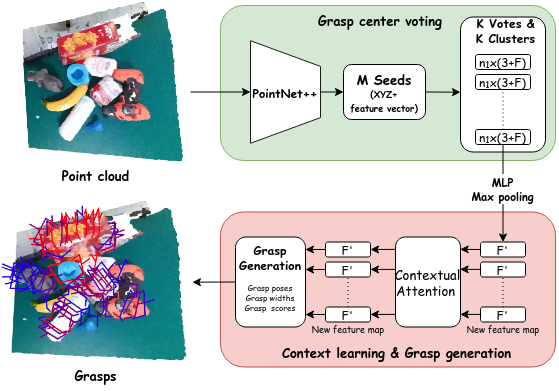
\includegraphics[width=0.8\linewidth]{figs/VoteGrasp.png}	
	\caption{VoteGrasp model using voting architecture and attention module for 6-DOF grasp detection in point cloud data. Our model conducts several self-attention modules discussed in section \ref{sec:attentions} following Hough voting network (\textcolor{cyan}{\cite{qi2019deep}}) to learn contextual information. Green grasps refer to highest quality grasps and red ones refer to lowest quality grasps.}
	\label{fig:VoteGrasp}
\end{figure*}

VoteGrasp is designed based on voting mechanism to overcome the obstacle of detecting grasps in occlusion and cluttered environments. Fig.\ref{fig:VoteGrasp} illustrates the overall architecture of VoteGrasp. Given a point cloud input of size $N\times3$, our method outputs a set of potential grasps, in which each grasp $G=(p,R,w,q)$ is accompanied by a center point $p=(x, y, z) \in \mathbb{R}^3$, gripper orientation $R \in SO(3)$, gripper width $w \in \mathbb{R}$, and grasp score $q \in [0,1]$. In terms of gripper estimation, we reformulate $R$ as in (\textcolor{cyan}{\cite{kehl2017ssd}}) instead of directly regressing it because of non-linearlity of the rotation space (\textcolor{cyan}{\cite{peng2019pvnet}}). 

\textbf{Backbone Network:} We take advantage of PointNet++ architecture as our backbone to extract geometric features. PointNet++ consists of set learning layers to combine features from multiple scales therefore able to enrich local features with increasing contextual scales. This backbone network prefers $M$ seed points and extracts high-dimensional features $\lbrace{s_i}\rbrace^{M}_{i=1}$ where $s_i=[x_i,f_i]$ is feature of a seed point specified by seed location in 3D space $x_i \in \mathbb{R}^{3}$ and feature vector $f_i \in \mathbb{R}^{F}$.

\textbf{Vote and Cluster:} The $M$ seed points are used as materials for computing votes for grasps. Each vote is characterized by a grasp center point and a feature vector for learning grasp. To obtain this, a multi-layer perceptron (MLP) containing fully connected layers, ReLU, and batch normalization is employed to compute $J$ votes per seed. This allows us to estimate multiple grasp poses for each object. We collect a set of votes $\lbrace \lbrace v_{ij} = [y_{ij}, g_{ij}] \in \mathbb{R}^{3+F}\rbrace^{M}_{i=1}\rbrace^{J}_{j=1}$. Here $v_{ij}$ is $j^{th}$ vote in $J$ set votes at $i^{th}$ point in $M$ seed points. $y_{ij}$ and $g_{ij}$ ($F$-dimensions) represent grasp center and feature vector learned for final grasp detection of vote $v_{ij}$ correspondingly. The next vital step is to cluster the votes by uniform sampling and finding neighboring votes within a certain Eclidean distance. Basing on a grasp center ${y_i}$ from a vote $\lbrace v_i=[y_i,g_i] \in \mathbb{R}^{3+F} \rbrace^{M \times J}_{i=1}$ calculated in previous step, we use iterative farthest point sampling (FPS) to select a subset of $K$ votes $\lbrace v_{ik} \rbrace^K_{k=1}$ in the neighborhood. A ball query finds $K$ neighboring votes $v_{ik}$ within a radius vacinity. The output are $K$ groups of vote sets of size $K \times n_k \times (3+F)$, where each group elects a grasp center and $n_k$ is number of neighbors of vote $v_{ik}$.

\textbf{Context learning:} In cluttered environments, grasping is inherently challenging because a successfull grasp has to be aware of both invisible object parts and potential collisions. The relationships between objects in the scene play an essential role in detecting collision-free grasps. Therefore, the correlations between objects and contextual information outside of interest regions are encoded into features to facilize this critical information to be learned. However, VoteNet (\textcolor{cyan}{\cite{qi2019deep}}) is originally designed to detect objects independently thanks to grouping votes which respond to one object centroid. Each cluster $C_k$ is fed into MLP layers to immediately regress its object class and bounding box. In our work, instead process each cluster instantly, we compute a new feature map by attaching relationship information between all clusters. Inspired by self-attention-based models (\textcolor{cyan}{\cite{vaswani2017attention}},\textcolor{cyan}{\cite{xie2018attentional}}, \textcolor{cyan}{\cite{wang2018non}}, \textcolor{cyan}{\cite{fu2019dual}}), we integrate a contextual module into our framework to acquire interdependencies between clusters. In more detail, votes $\lbrace v_i = [y_i,g_i] \in \mathbb{R}^{3+F} \rbrace ^{n_k}_{i=1}$ in each clusters $K$ are firstly fed into a MLP and max-pooling layer to aggregate a single feature vector $C_k \in \mathbb{R}^{F'}$. Summarizing all these single vector of $K$ clusters, we gain a feature map $C=[C_1;C_2;...;C_K] \in \mathbb{R}^{F \times F'}$. The next step is to learn correlations between clusters in $C$ by conducting a context learning module. New rich contextual feature map is generally formulated as Eq.\ref{eq:VoteGrasp_compute_context}. The particular form of formulation depends on the certain attention module applied and it is deeply discussed in \ref{sec:attentions}.
%%%%%%%%%%%%%%%%%%%%%%%%
\begin{align}
\label{eq:VoteGrasp_compute_context}
C^{context}_i = \sum_{}^{} f(\theta(C_i), \psi(C_j)) \odot g(C_j) \
\end{align}
%%%%%%%%%%%%%%%%%%%%%%%%
Where $\theta(.)$, $\psi(.)$, $g(.)$ are learnable transformations and $f(i)$ is relation function to encode relation between all positions. The widespread relation function is the dot-product family, but in our research, we further examine other relation functions. The new feature map $C_{context} = [C^{context}_1; C^{context}_2;...;C^{context}_K \in \mathbb{R}^{K \times K'}$ has same size with input feature. By leveraging self-attention mechanism, our network enables features of different clusters to communicate with each other. The contribution and effectiveness of the context learning module will be thoroughly illustrated in later sections.

\textbf{Grasp Detection:} New feature map $C^{context}$, which is enlarged with relationships between clusters, is then passed through a multi-layer perceptron (MLP) network to detect a ranked list of grasps $G=(p,R,w,q)$. More specifically, our model detects a grasp center $p=(x,y,z) \in \mathbb{R}^3$, gripper orrientation $R \in SO(3)$, gripper width $w \in \mathbb{R}$, and grasp quality $q \in [0,1]$. The MLP is implemented with 3 fully connected layers and two first of them are followed by batch normalization and ReLU. The last one - the prediction layer has $5+V+2A$ channels, in particular they are 3 grasp center regression values, 1 gripper width regression value, 1 grasp cinfidence regression value, $V$ viewpoint scores, $A$ angle scores (in-plane rotation), and $A$ angle residual regression values (in-plane rotation). $V$ and $A$ represent the numbers of sampled viewpoints and in-plane rotations respectively.

\textbf{Loss Function:} The grasp detecton is supervised with multi-task loss:
%%%%%%%%%%%%%%%%%%%%%
\begin{align}
L_{votegrasp} = L_{vote} + L_{grasp} \
\end{align}
%%%%%%%%%%%%%%%%%%%%%
The VoteGrasp loss $L_{votegrasp}$ includes a voting loss $L_{vote}$ and a grasp estimation loss $L_{grasp}$. Voting loss is built as a regression loss:
%%%%%%%%%%%%%%%%%%%%%
\begin{align}
L_{vote} = \frac{1}{M_s} \sum_{i}^{} {\lVert y_i-c^g_i \rVert}_H \cdot \mathds{1}(x_i)   \
\end{align}
%%%%%%%%%%%%%%%%%%%%%
Where $M_s$ denotes the total number of seeds on the object surface, $c^g_i$ is the closest ground truth grasp center, ${\lVert \cdot \rVert}_H$ is the Huber norm and $\mathds{1}(\cdot)$ is a binary function that indicates whether or not a seed point $s_i$ belongs to an object. In terms of grasp loss function, it is defined as follows: 
%%%%%%%%%%%%%%%%%%%%%
\begin{align}
L_{grasp} = L_center + \alpha L_{rot} + \beta L_{width} + \gamma L_{score} \
\end{align}
%%%%%%%%%%%%%%%%%%%%%
The grasp loss consists of a grasp center loss (regression) $L_{center}$, a rotation loss $L_{rot}$, a gripper width loss (regression) $L_{width}$, and a grasp confidence score (regression) $L_{score}$. The grasp center loss is conducted with two elements $L_{center} = L_{viewpoint} + L_{in-plane}$. While $L_{viewpoint}$ represents for viewpoint classification, the in-plane rotation estimation is designed as a combination of classification and regression as $L_{in-plane} = 0.1L_{angle-cls}+L_{angle-reg}$ (\textcolor{cyan}{\cite{qi2018frustum}}). We conduct $L1$-smooth loss (\textcolor{cyan}{\cite{ren2015faster}}) for all regression ingredients and standard cross entropy for classification losses. 

\vspace{0.2cm}

\subsection{Attentions}
\label{sec:attentions}
In this section, we want to thoroughly discuss attention modules that we employ in our research. This provides insights into how attention mechanism operates in each module and its potentiality in collision-free grasp detection. We will examine how differently they capture interdependencies inside feature map and operate relation function. The detail of implementation and results of plugging each module into VoteGrasp are evaluated in section 4.
%%%%%%%%%%%%%%%%%%%%%%%%%%%%%%%%%%%%%%%%%%%%%%%%%%%%%%%%%%%%%%%%%%%%%%%%%%%%%%

\textbf{Non-local} (\textcolor{cyan}{\cite{wang2018non}}):
The idea of this method is inspired by non-local means algorithm (\textcolor{cyan}{\cite{buades2005non}}) for denoising images. Non-local means computes the denoised value at a position as a weighted average of all pixels in the image. The family of weights between two pixels depends on the similarity between them. Non-local Neural Network forms this idea into deep stacks of convolutional operations to capture long-range dependencies in sequential data. 
%%%%%%%%%%%%
\begin{gather}
	\label{eq: non_local_comp_response}
	y_i = \frac{1}{C(x')} \sum_{\forall j}^{} f(x_i, x'_j)g(x'_j) \\
	\label{eq: non_local_comp_z}
	z_i = W_z y_i + x_i \
\end{gather}

%%%%%%%%%%%%%%%%%%%%
\begin{figure}
 	\centering	
 	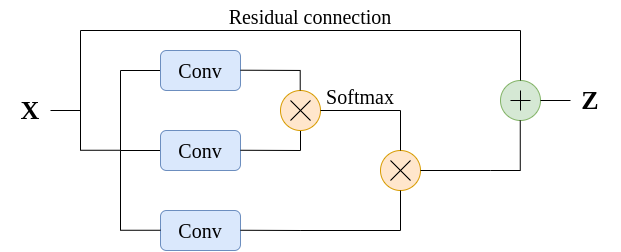
\includegraphics[width= 0.8\linewidth]{figs/non_local_diagram.png}
 	\caption{Non-local block diagram. The input feature is transformed by $1 \times 1 \times 1$ convolutions. $``\otimes"$ denotes matrix multiplication, and $``\oplus"$ denotes element-wise sum.}
 	\label{fig:non_local}
\end{figure}
%%%%%%%%%%%%%%%%%%%%

Eq.\ref{eq: non_local_comp_response} computes responses $y$ based on relationships between different locations. It is proved to be a generic non-local operation due to the fact that it takes all positions $\forall j$ into consideration. $x$ is the input signal, which could be images, videos, but often features. To reduce the computation, the authors use $x'$ as a subsampled version of $x$ by using pooling technique (max pooling). $z$ is the output feature that has variable sizes as input $x$ and therefore keeps the positional correspondences of input data to be intact. $i$ is the index of an output position and $j$ is the index that enumerates all positions. $f$ is the pairwise function (relation function) that represents the relationship between $i$ and all $j$. In this research, authors examine the use of several pairwise functions of Gaussian, Embedded Gaussian, Dot product, Concatenation, or simply done by matrix multiplication as shown in Fig.\ref{fig:non_local}. $g$ represents the input signal at position $j$. $C(x')$ is normalizing factor and softmax function is used here. The non-local operation in Eq.\ref{eq: non_local_comp_response} is wrapped into a non-local block by adding residual connection component “$+x_{i}$” as define in Eq.\ref{eq: non_local_comp_z}. This residual connection facilitates non-local block to insert a new one into the pre-trained model and does not interrupt its initial weight matrix $W_z$. This lightweight and easy-to-implemented block is plugged into many architectures such as classification, and segmentation to learn “where” they should pay more attention.

%%%%%%%%%%%%%%%%%%%%%%%%%%%%%%%%%%%%%%%%%%%%%%%%%%%%%%%%%%%%%%%%%%%%%%%%%%%%%

\textbf{Criss-cross} (\textcolor{cyan}{\cite{huang2019ccnet}}):
Similar to Non-local block, this building block is conducted to capture pixel-wise dependencies between all positions in images. Non-local block performs significantly in classification tasks. Nonetheless, confronting dense prediction tasks such as segmentation, which heavily requires high resolution of feature maps, pressures this method to reveal its weakness in consuming huge computation complexity and GPU memory. Therefore, criss-cross attention module harvests contexts in images’ criss-cross paths to obtain dense contextual information while keeping feature maps to be lightweight. In other words, this architecture prefers aggregating contextual information in horizontal and vertical directions to averaging all pixels. As a result, this is $11\times$ faster and saves $85\%$ FLOPs in comparison with non-local block. Given an input feature map $X \in \mathbb{R}^{H \times W}$, non-local produces $H \times W$ weights, while criss-cross method generates $H+W-1$ weights. However, the pixels not in a criss-cross path are still absent in the aggregation of one pixel. The authors use $(R=2)$ loops of criss-cross attention modules to guarantee full-image pixels are harvested to produce feature maps with dense contextual information. Adding this block to architectures allows them to boost their performance in both result accuracy and inference time.
%%%%%%%%
\begin{figure*}[h!]
 	\centering	
 	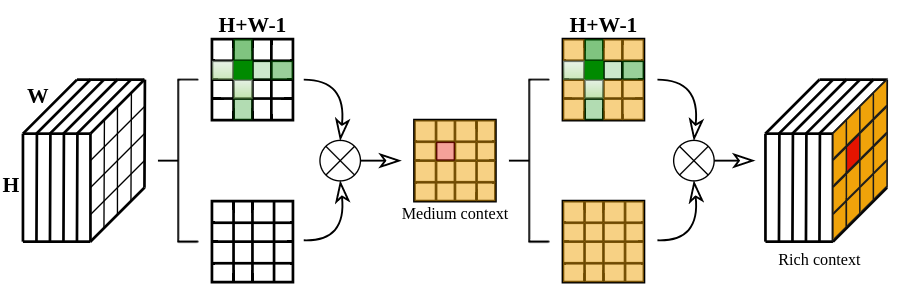
\includegraphics[width= 0.8\linewidth]{figs/criss-cross.png}
 	\caption{Criss-cross block architecture captures interdependencies in vertical and horizontal directions. The block consists of two criss-cross operations to capture interdependencies of all pixels. The differences in shades of green represent different meanings that a pixel contributes to the target pixel (red). Similarly, the differences in shades of yellow illustrate the wealth of contextual information.}
 	\label{fig:criss-cross}
\end{figure*}
%%%%%%%%

%%%%%%%%%%%%%%%%%%%%%%%%%%%%%%%%%%%%%%%%%%%%%%%%%%%%%%%%%%%%%%%%%%%%%%%%%%%%%%

\textbf{Squeeze-and-Excitation (SE)} (\textcolor{cyan}{\cite{hu2018squeeze}}):
This research strengthens the power of the convolutional operator by exploiting the interdependencies between the channels of convolutional features. Instead of focusing on spatial relationships like non-local and criss-cross network, it looks into another aspect – the relationship between channels. This block consists of two modules: Squeeze and Excitation. Squeeze operation aims to produce channel descriptors that embed global distribution feature responses. Using global average pooling allows this module to generate channel-wise statistics $y$. Given a input feature map $X \in \mathbb{R}^{H \times W \times C}$ and $x_c \in R^{H \times W}$ is the feature map at $c^{th}$ channel. A $c^{th}$ element of $y$ is calculated at $c^{th}$ channel of input data as following formula. Thus, $Y \in \mathbb{R}^C$ is a collection of average representation of all pixels of all channels.
%%%%%%%%
\begin{figure*}[h!]
 	\centering	
 	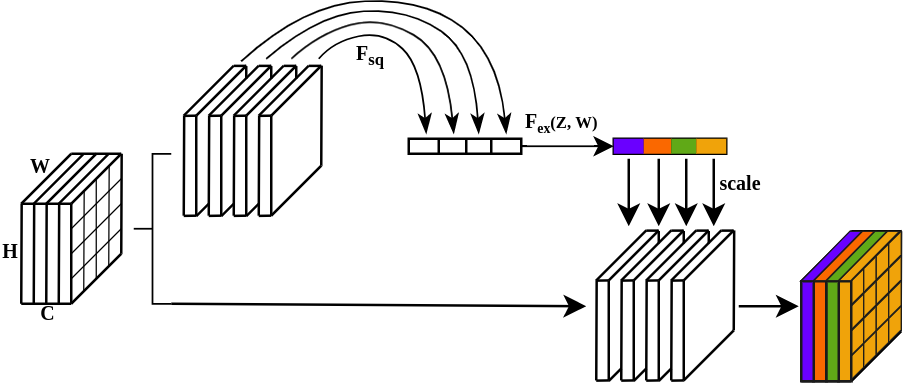
\includegraphics[width= 0.8\linewidth]{figs/SE.png}
 	\caption{Squeeze-and-Excitation block focuses on the channel relationship of input feature. Different colors depict the distribution of channel information.}
 	\label{fig:SE}
\end{figure*}
%%%%%%%%%%%%%%%%%%%
%%%%%%%%%%%%%%%%%%
\begin{gather}
\label{eq:SE_F_squeeze}
y_c = F_{sq}(x_c)= \frac{1}{H \times W}\sum_{i=1}^{H} \sum_{j=1}^{W}x_c(i,j)\\
\label{eq:SE_F_excitation}
s=F_{ex}(y, W)\\
z_c = s_c y_c \
\end{gather}

The next operation – Excitation – aggregates the information in the previous one. This one focuses on totally gathering channel-wise dependencies. To obtain this purpose, it makes use of a simple self-gating mechanism that takes embedding features, which is the output of Squeeze operation, as input to generate per-channel modulation weights $s \in \mathbb{R}^C$ as Eq.\ref{eq:SE_F_excitation}. At the end of the operation, input feature map $X$ is rescaled with modulation weight $s$. The final feature map $Z \in \mathbb{R}^{H \times W \times C}$ can indicate to what extent each channel is informative. This output map can be used by subsequent layers and help them learn “what” they should look at. This block is proved to be insertable to neural network architectures to boost their performance in scene classification and object detection.

%%%%%%%%%%%%%%%%%%%%%%%%%%%%%%%%%%%%%%%%%%%%%%%%%%%%%%%%%%%%%%%%%%%%%%%%%%%%%%%%
\textbf{Compact Generalize Non-local (CGNL) (\textcolor{cyan}{\cite{yue2018compact}})}:
This compact block is designed to achieve high accurate object recognition, especially in fine-grained objects and actions. The research notices the lack of considering interactions between positions across channels of non-local module or even criss-cross module. They solely capture dependencies between spatial pixels and temporal frames by merging channels. Hence, they pay more attention to object part relations but neglect crucial clues for recognizing actions - the interactions between objects, which correspond to different channels. Although SE network mentioned previously learns interdependencies between channels, it treats all positions in a similar way by global averaging as Eq.\ref{eq:SE_F_squeeze}. Therefore, to acquire long-range correlations as well as interactions, CGNL learns correlations among all elements across the channels by merging channels into positions. It could be clearly understood that this method fuses channel information into positional features. The input feature map $X \in \mathbb{R}^{H \times W \times C}$ is firstly divided into $G$ groups and each sub-feature map $X'$ contains $C' = C/G$ channels. In comparison with \ref{eq: non_local_comp_response}, CGNL reshapes the output of transformation function to $HWC'-D$ vector column as Eq.\ref{eq:CGNL_reshape_transform} to fuses channel into position.
%%%%%%%%%%%%
\begin{gather}
\label{eq:CGNL_reshape_transform}
\theta(X') = vec(X'W_{\theta}) \in \mathbb{R}^{HWC'} 	\\
\phi(X') = vec(X'W_{\phi}) \in \mathbb{R}^{HWC'}		\\
g(X') = vec(X'W_g) \in \mathbb{R}^{HWC'}				\\
\label{eq:CGNL_compute_response}
vec(Y') = f(\theta(X'), \phi(X'))g(X') \
\end{gather}
%%%%%%%%%%%%%
Pairwise function (relation function) $f:\mathbb{R}^{HWC'}\times\mathbb{R}^{HWC'} \rightarrow \mathbb{R}^{HWC'}\times\mathbb{R}^{HWC'}$ can distinguish pairs of same location but at different channels so that can enrich greatly feature map for action recognizing or fine-grained object classification. Each feature map $Y'$ computed from each group is then concatenated along the channel dimension to restore $Y$. By informing this formulation, this module produces competitive or state-of-the-art result on benchmark datasets.

%%%%%%%%%%%%%%%%%%%%%%%%%%%%%%%%%%%%%%%%%%%%%%%%%%%%%%%%%%%%%%%%%%%%%%%%%%%%%%%
\textbf{Dual Attention Network (DANet)} (\textcolor{cyan}{\cite{fu2019dual}}):
Methods discussed above solely use either position attention or channel attention. While position attention selectively calculates the feature of each pixel by a weighted average of all pixels, channel attention selectively emphasizes interdependencies between channels among all channel maps. Despite the fact that dual attention network further improves the discriminative representation of feature map by applying self-attention mechanism for both positional and channel dependencies. To obtain this, it feeds input data through two parallel modules of position attention and channel attention to capture long-range contextual information. The attention module commonly operates as the attentional component in previously reviewed methods. In the research, the authors examine the contribution of each attention module to the precise segmentation results. They perceive that the absence of any module would harm the accuracy of prediction task. Using both modules outcome highest Mean IoU indicator in scene segmentation among applying none, solely position, or solely channel attention. It could be interpreted that dual attention network allows architectures to emphasize “where” and “what” to be most meaningful. 
%%%%%%%%%%%%%%%%%%%%%%%%%%%%%%
\begin{figure*}[h!]
	\centering
	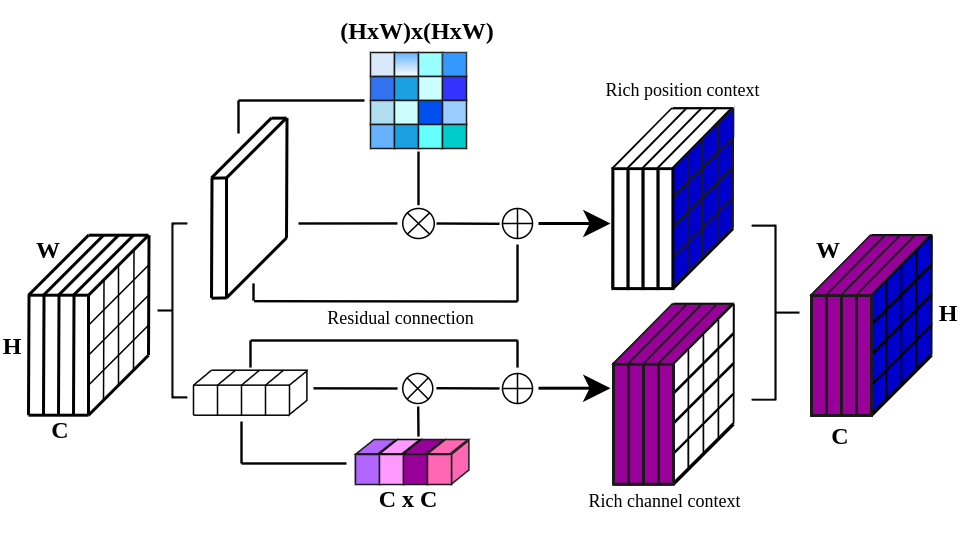
\includegraphics[width = 0.65\linewidth]{figs/Dual_attention.png}
	\label{fig:Dual_attention}
	\caption{Architecture of dual attention network includes two module of position attention and channel attention. The output feature is rich of position context and channel context.}
\end{figure*}

%%%%%%%%%%%%%%%%%%%%%%%%%%%%%%%%%%%%%%%%%%%%%%%%%%%%%%%%%%%%%%%%%%%%%%%%%%%%%%
\textbf{Convolutional Block Attention Module (CBAM)} (\textcolor{cyan}{\cite{woo2018cbam}}):
Similar to DANet for upgrading discriminative features, this module employs both spatial and channel information for attention mechanism. However, this one is different from DANet that it conducts spatial and channel attention modules in a sequential arrangement. Research also investigates diverse combinations of these two attention modules: placing the channel module first, placing the spatial module first, placing them in parallel, and placing them in sequence. Practical experiments reveal that organizing the spatial module following up channel module achieves the lowest error rate. Moreover, plugging into pre-existing architecture such as MobileNet, Faster-RCNN, StairNet, SSD, and CBAM reach slight successful detection in comparison with Squeeze-and-Excitation block.

%%%%%%%%%%%%%%%%%%%%%%%%%%%%%%%%%%%%%%%%%%%%%%%%%%%%%%%%%%%%%%%%%%%%%%%%%%%%%%
\textbf{Point-Attention} (\textcolor{cyan}{\cite{feng2020point}}):
Attention mechanism obviously demonstrates its strength in upgrading the performance of prediction architectures. However, most of them are being used for 2D data due to applying for 3D data is not straightforward. 3D point clouds inherently are irregular, sparse, unordered, and non-grid structures. Immediately exploiting the above methods for 3D point clouds might require voxelization which losses informative components of input data. Information about neighbors is crucial in attention operation so that the process of converting point clouds into a discrete grid appears to be destructive to final results. Therefore, Point Attention Network (PAN) is introduced to employ self-attention mechanism while directly dealing with 3D point clouds. It captures neighbors’ contextual correlation in multi-directions to enrich local shape features by layers called Local Attention-Edge Convolution (LAE-Conv). Then, the following point-wise spatial attention module obtains long-range spatial contextual dependencies to achieve more precise segmentation. In 3D point set, some points far away from a particular point pi appear to be not meaningful to the representation of $p_i$. Therefore, PAN conducts LAE-Conv to search for meaningful neighbors beforehand to enhance the local representation of point $p_i$. A ball space of a central point with $r$ radius is formed and divided into $K$ uniform bins. Radius $r$ is selected to ensure that each bin contains at least $m$ neighbors and only $m$ nearest neighbors contribute to the representation of the central point. Experiments yield $K=16$ and $m=1$ gain the highest accuracy. In comparison of this searching operation with other methods, we have some clear discussion. PointNet++ searches neighbors within a ball query radius. A PointNet-based hierarchical network separately processes local points. It, however, ignores the relationships between points. Moreover, the ball query selects all points inside the ball which would be tricky if the number of neighbors is small. On the other hand, although K-nearest neighbors (KNN) outputs a fixed number of neighbors, it does not guarantee that neighboring information comes from all directions. Neighborhood points found by LAE-Conv are not treated equally, the contribution of neighbors is computed by attention mechanism and the updated features of central point $p_i$ are aggregated with respect to $K$ neighbors.
\begin{gather}
\label{eq:alpha_point_attention}
\alpha_{ij}= softmax(a(W(p_j - p_i))) \\
\label{eq:p_i_point_attention}
p'_i = \sum_{j \in N_{p_i}} \alpha_{ij} W_{p_j}\
\end{gather}

Where $p_i$ is central point and its neighbor $p_j$. $\alpha_{ij}$ is weight coefficient of point $p_j$ to contribute to $p_i$ and it is normalized by softmax function. $W$ is a learnable weight matrix that transforms the input point to a higher-level local feature. $(p_j-p_i)$ is a function to transform neighbor to local coordinate systems. $p'_i$ is the higher-level feature of central point $p_i$. The wealthy representation of local geometric features extracted from LAE-Conv is fed into Point-wise spatial module to further capture long-range contextual information. This is obtained by the prevalent attention mechanism as shown in Fig.\ref{fig:point_attention}. Weight map $S$ is computed weight function added softmax normalization. The presence of PLAE in Fig.\ref{fig:point_attention} refers to residual connection. Practicing PAN on challenging benchmarks proves its ability to achieve 3D object detection is competitive with other state-of-the-art methods.
%%%%%%%%%
\begin{figure*}[h!]
\centering
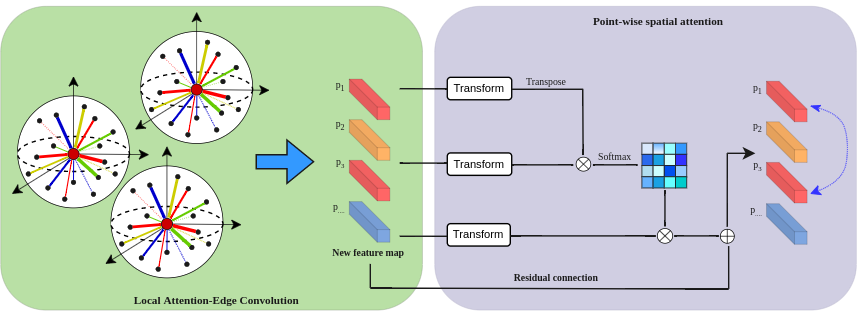
\includegraphics[width= \linewidth]{figs/Point_attention.png}
\caption{Local-global architecture of Point-attention block contains Local Attention-Edge Convolution module and Point-wise spatial attention. The first module searches a target point's 16 neighbors within a ball and computes a new feature map, which is enriched with geometric information of neighbors. The thickness of lines connecting the center point to neighbors refers to different contributing values. After enlarging local representation, the second module captures global correlations.}
\label{fig:point_attention}
\end{figure*}

%%%%%%%%%%%%%%%%%%%%%%%%%%%%%%%%%%%%%%%%%%%%%%%%%%%%%%%%%%%%%%%%%%%%%%%%%%%%%%
\textbf{Point Transformer} (\textcolor{cyan}{\cite{zhao2021point}}):
A self-attention-based backbone for diverse tasks with 3D point clouds such as object classification, object part segmentation, and semantic segmentation. The research explores the performance of two type of attention operation: scalar attention (\textcolor{cyan}{\cite{vaswani2017attention}}) and vector attention (\textcolor{cyan}{\cite{zhao2020exploring}}) and adding position encoding element as well. The attention layer of this method can be represented as follow.
%%%%%%
\begin{align}
\label{eq: point_transformer}
y_i= \sum^{}{} \rho(\gamma(f(x_i, x_j) +\varepsilon) \odot (g(x_j) +\varepsilon)) \
\end{align}
%%%%
Where $y_i$ is responses based on different locations, $\rho$ is the normalizing function, $\gamma$ is the mapping function to transform the output of the relation function to right dimensionality, and $\varepsilon$ is the position encoding element. To clearly understand the examining scalar attention and vector attention, we look closer into relation function $f$. There are two forms of attention operator: pairwise self-attention and patchwise self-attention. 
\begin{itemize}
	\item The more common pairwise self-attention, in which weight computation $f(x_i,x_j)$ is computed by aggregating all feature vectors of positions $x_i, x_j$ within whole image as Eq.\ref{eq: point_transformer}(without $\gamma$ and $\varepsilon$ ingredients). The dimensionality of relation function output depends on the form of relation function $f$. The pre-dominant formulation is dot-product attention that produces output with dimensionality equals to 1. This construction shares its output across all channels and does not adapt the attention weights at different channels. The specific choice of dot-product is termed scalar attention. The other cases of relation function such as summation, subtraction, and Hadamard production produce vector output (\textcolor{cyan}{\cite{zhao2020exploring}}) can be additionally processed to map right dimensionality to input features by $\gamma$ function. Therefore, vector weights can vary along the channel dimensions, and it is termed vector attention. In Point Transformer, subtraction relation is selected for relation function to apply vector attention. Experiments yield that using vector attention (Subtraction relation) outperforms using scalar attention (Dot-product relation). 
%%%%%%%%%%%%%%%%%%%%%%%%%%%%%%%%%%%%%%
\begin{align}
\alpha(x_i,x_j)=\gamma(f(x_i, x_j))													\\
\textbf{Dot-product:} \; f(x_i, x_j) = \varphi(x_i)^{\top} \psi(x_j) 			\\
\textbf{Summation:} \; f(x_i,x_j) = \varphi(x_i) + \psi(x_j) 				\\
\textbf{Subtraction:} \; f(x_i,x_j) = \varphi(x_i) - \psi(x_j) 				\\
\textbf{Hadamard product:} \; f(x_i,x_j) = \varphi(x_i) \odot \psi(x_j) 			\
\end{align}
%%%%%%%%%%%%%%%%%%%%%%%%%%%%%%%%%%%%
	\item Another form of attention is patchwise attention, in which the input of relation function is the patch of feature vectors $x_{R(i)}$ instead of feature vector $x(i)$ at a particular position. Moreover, the output of wight computation function alpha(xR(i)) is a tensor of same spatial dimensionality as the patch $x_{R(i)}$. Thus, patchwise attention inherently is vector attention. Several selections for relation function are Star-product, Clique-product, Concatenation (\textcolor{cyan}{\cite{zhao2020exploring}}).
	\item \textbf{Position encoding.} In pairwise attention, feature vectors $x(j)$ are processed independently so that the weight computation cannot leverage information from any location except for $i$ and $j$. Therefore, position encoding facilizes augmenting feature maps with position information. The importance of position encoding is examined in experiments suggest that applying relative position encoding for both attention $(f(x_i,x_j) + \varepsilon)$ and feature $(g(x_j)+\varepsilon)$ accomplishes the highest performance.
\end{itemize}

%
\section{Evaluation}
\label{sec:Experiments}

In this section, we would like to answer the following questions: (1) How do attention modules would affect the performance of grasp detection? What sort of attention modules is suitable for 3D point cloud data? How well do the learned models generalize to novel object categories? To answer the above questions, we conduct the experiments of grasp detection on the public dataset GraspNet-1Billion \cite{fang2020graspnet}. This is a large-scale grasp dataset collected from cluttered scenes considering multi-object-multi-grasp setting. The objects in GraspNet-1Billion have varying shapes, textures, sizes, materials, and underlying different occlusion conditions. Hence, it can be used to evaluate robustness to occlusion and the generalization ability of trained models.

%%%%%%%%%%%%%%%%%%%%%%%%%%%%%%%%%%%%%%%%%%%%%%%%%%%%%%%%%%%%%%%

\begin{figure*}[h!]
  \centering  
    \begin{subfigure}[b]{0.25\linewidth}
    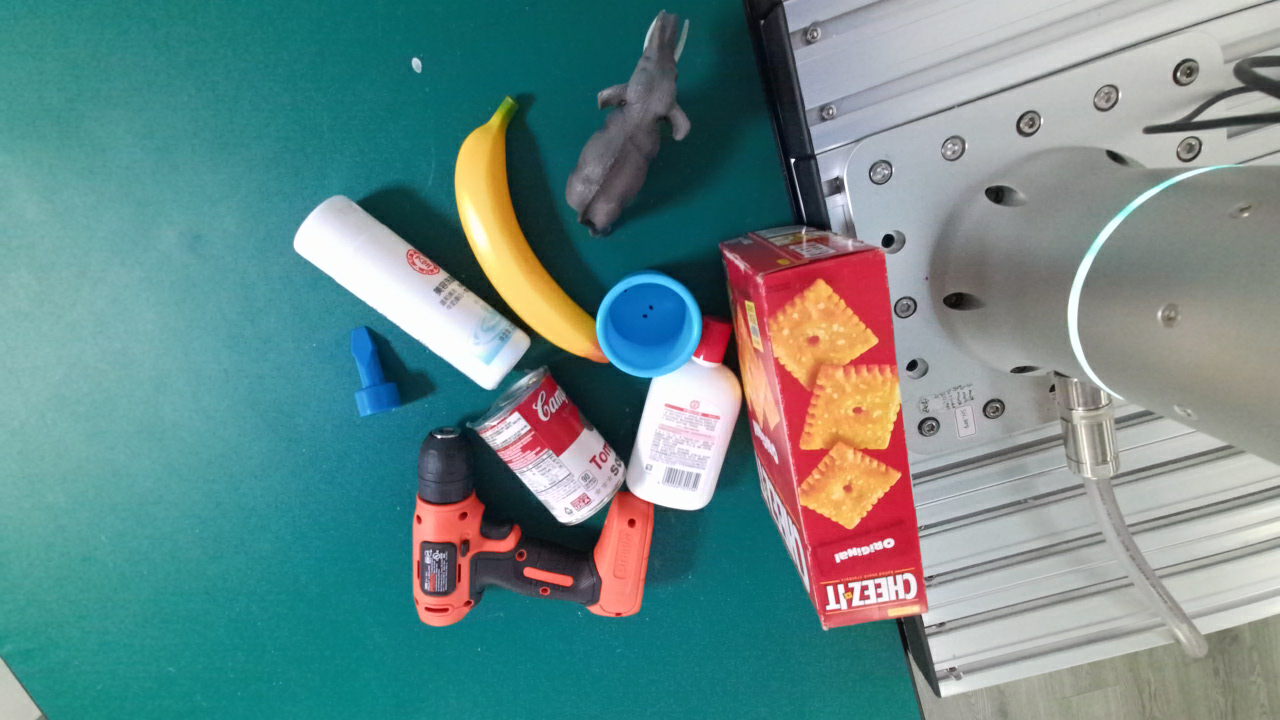
\includegraphics[width=5cm]{figs/Attention_module_results/color.png}
  \caption{}  
  \end{subfigure}
  
  %%%%%%%%%%%%%%%%%%%%%%%%%%%%%%%
  
  \begin{subfigure}[b]{0.32\linewidth}
    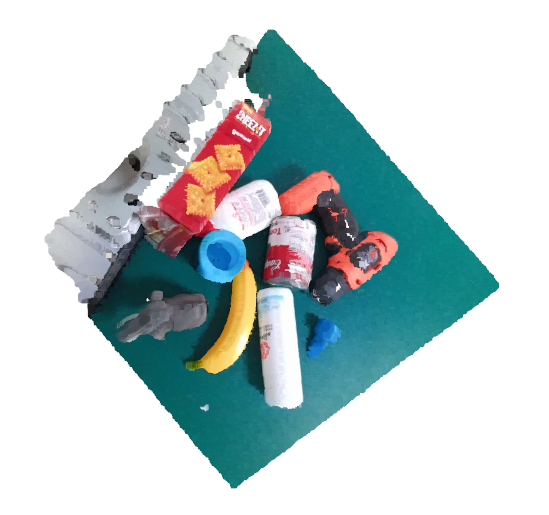
\includegraphics[width=5cm]{figs/Attention_module_results/pointcloud.png}
  \caption{}  
  \end{subfigure} 
  \begin{subfigure}[b]{0.32\linewidth}
    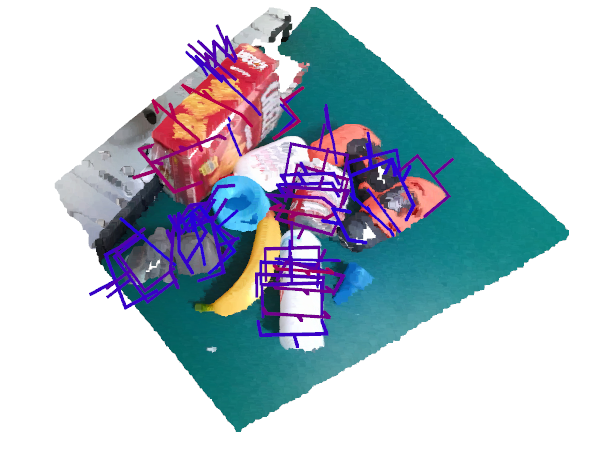
\includegraphics[width=5cm]{figs/Attention_module_results/Non-local.png}
    \caption{} 
  \end{subfigure} 
  \begin{subfigure}[b]{0.32\linewidth}
    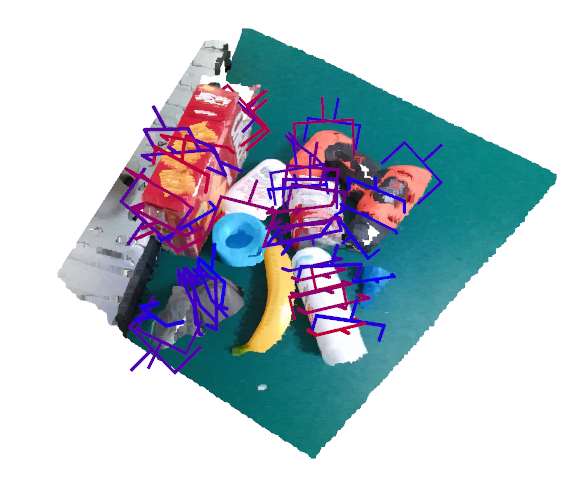
\includegraphics[width=5cm]{figs/Attention_module_results/Criss-cross.png}
  \caption{}  
  \end{subfigure}
  
  %%%%%%%%%%%%%%%%%%%%%%%%%%%%%%%%%%%%%%%%%%%%%%%%
  
    \begin{subfigure}[b]{0.32\linewidth}
    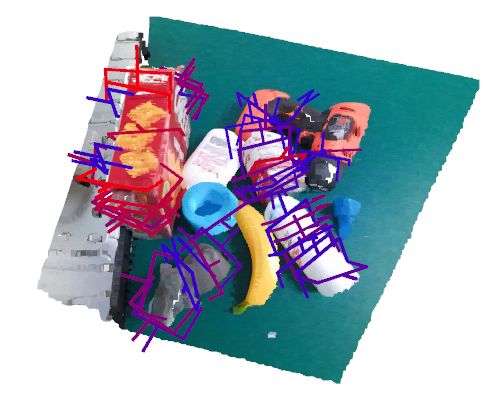
\includegraphics[width=5cm]{figs/Attention_module_results/SE.png}
  \caption{}  
  \end{subfigure}   
  \begin{subfigure}[b]{0.32\linewidth}
    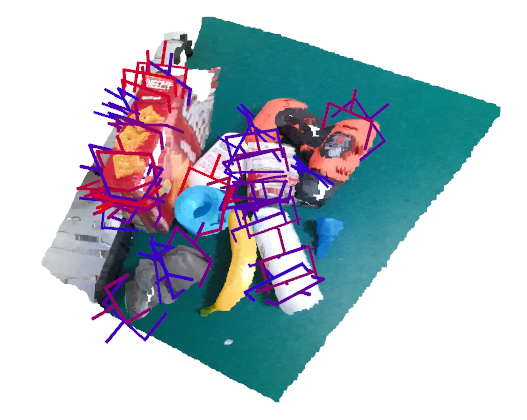
\includegraphics[width=5cm]{figs/Attention_module_results/CGNL.png}
    \caption{} 
  \end{subfigure}   
      \begin{subfigure}[b]{0.32\linewidth}
    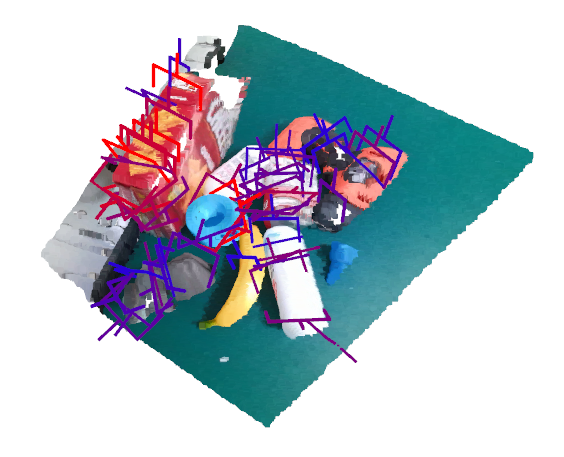
\includegraphics[width=5cm]{figs/Attention_module_results/DANet.png}
    \caption{} 
  \end{subfigure} 
  
   %%%%%%%%%%%%%%%%%%%%%%%%%%%%%%%%% 
   
    \begin{subfigure}[b]{0.25\linewidth}
    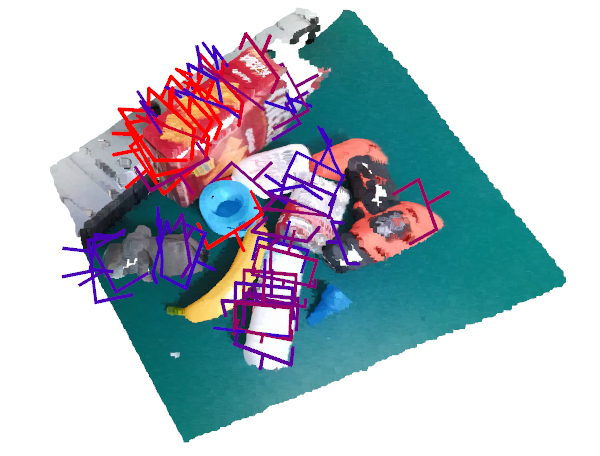
\includegraphics[width=5cm]{figs/Attention_module_results/CBAM.png}
    \caption{} 
  \end{subfigure} 
    \begin{subfigure}[b]{0.32\linewidth}
    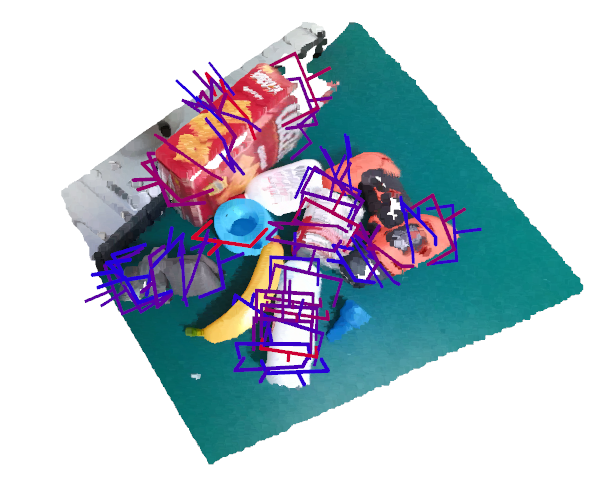
\includegraphics[width=5cm]{figs/Attention_module_results/Point-Attention.png}
    \caption{} 
  \end{subfigure} 
    \begin{subfigure}[b]{0.32\linewidth}
    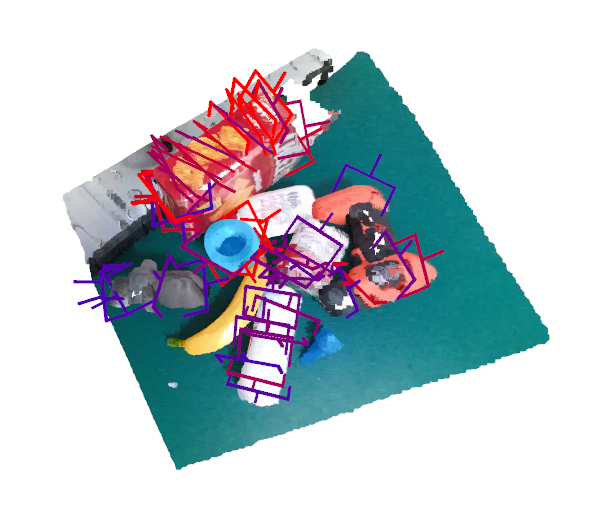
\includegraphics[width=5cm]{figs/Attention_module_results/Point_Transformer.png}
    \caption{} 
  \end{subfigure}
  
  \caption{Examples of input point clouds and predicted grasps from VoteGrasp combining with different attention module; (a) experiment objects; (b) input point cloud; (c) Non-local; (d) Criss-cross; (e) Squeeze-and-Excitation; (f) Compact Generalized Non-local; (g) Dual Attention Network; (h) Convolution Block Attention Module; (i) Point attention; (j) Point transformer. The different intensity of grasp color denotes the confident score of grasps. Red refers to the highest quality grasps and blue refers to the lowest ones.}
  \label{fig:grasp_pred_result}
\end{figure*}

%%%%%%%%%%%%%%%%%%%%%%%%%%%%%%%%%%%%%%%%%%%%%%%%%%%%%%%%%%%%%%%

\subsection{GraspNet-1Billion}

The GraspNet-1Billion (\textcolor{cyan}{\cite{fang2020graspnet}}) consists of 97,280 RGB-D images captured from 190 cluttered scenes. The dataset provides over one billion grasp poses for 88 objects presented in the scenes and an accurate 3D mesh model of each object is available as well. Besides, it also provides relevant information including camera poses, 6D object poses, object masks, and bounding boxes for all frames. The rich annotations allow us to generate ground truth votes and grasp configurations easily. Following (\textcolor{cyan}{\cite{fang2020graspnet}}) we split the dataset into 100 scenes for training and 90 scenes for testing. To evaluate model generalizability, the test sets are divided into 30 scenes with novel objects, 30 for unseen but similar objects, and the rest for seen objects.

\subsection{Implementation}

%%%%%%%%%%%%%%%%%%%%%%%%%%%%%%%%%%%%%%%%%%%%%%%%%%%%%%%%%%%

\begin{table}[h]
\caption{Layer parameters of the PointNet++ (\textcolor{cyan}{\cite{qi2017pointnet++}}) based feature learning network.}
\label{tab:layer_specs}
\begin{center}
\begin{tabular}{|l|c|c|}
\hline
layer name & input layer & layer params \\
\hline
SA1 & point cloud & (2048,0.025,[64,64,128]) \\
SA2 & SA1  & (1024,0.05,[128,128,256]) \\
SA3 & SA2 & (512,0.1,[128,128,256]) \\
SA4 & SA3 & (256,0.2,[128,128,256]) \\
FP1 & SA3, SA4 & [256,256] \\ 
FP2 & SA2, SA3 & [256,256] \\
\hline
\end{tabular}
\end{center}
\end{table}
%%%%%%%%%%%%%%%%%%%%%%%%%%%%%%%%%%%%%%%%%%%%%%%%%%%%%%%%%%%

In our implementation\footnote{Our code and other materials are available at \url{https://github.com/hoangcuongbk80/NovelVoteGrasp}}, we randomly choose $N$=50k points from each raw point cloud. We then apply the PointNet++ (\textcolor{cyan}{\cite{qi2017pointnet++}}) based feature learning network, which has 4 set abstraction layers (SA) and 2 feature propagation layers (FP). The detailed layer parameters are shown in Table~\ref{tab:layer_specs}. The FP2 outputs $M=1024$ seeds with $F=256-dim$ features and 3D coordinates that will be transformed to votes. The voting module generates $J=10$ votes per seed with an MLP layer spec: $[256, 256, 259 \times 10]$. In the attention module, we form $K=1024$ clusters and output a new feature map $C_{context} \in K \times F'$ where $K=1024, F'=128$. In the last step, 1024 grasps are detected from the new feature map. The prediction layer has $5 + V + 2A$ channels where $V=120$, and $A=6$.

The implementations are realized by PyTorch and Python platforms on one Nvidia GeForce RTX 2080 Ti 10GB GPU using CUDA and Linux operating system. All the experiments adopt similar training settings. The networks are trained from scratch in an end-to-end manner. We train each model over 200 epochs with stochastic gradient descent using a batch size of 8 and the Adam optimizer with a learning rate of 0.001.

\subsection{Metrics}

To evaluate the performance of grasp detection, we follow prior work (\textcolor{cyan}{\cite{fang2020graspnet}}) and report results using $Precision@k$. This metric measures the precision of top-k ranked grasps. We first check whether a predicted grasp ($G_{p}$) is true positive or not. It is considered a true positive only if the grasp satisfies three conditions: (i) there is an object inside the gripper; (ii) it is collision-free; (iii) the grasp is antipodal under a given friction coefficient $\mu$. The third condition is computed based on the prior works (\textcolor{cyan}{\cite{ten2017grasp, fang2020graspnet}}). We let $AP_{\mu}$ denote the average $Precision@k$ for $k$ ranges from 1 to 50 given a friction coefficient $\mu$. We report the average of $AP_{\mu}$ with $\mu = \left\lbrace 0.2,0.4,0.6,0.8,1.0 \right\rbrace $, denoted as \textbf{AP}.

\subsection{Results}

%%%%%%%%%%%%%%%%%%%%%%%%%%%%%%%%%%%%%%%%%%%%%%%%%%%%%%%%%%%
\begin{table}[h]
\caption{Inference Time of VoteGrasp with different attention modules, evaluated on GraspNet-1Billion (\textcolor{cyan}{\cite{fang2020graspnet}}) dataset.}
\label{tab:real_ex}
\begin{center}
\begin{tabular}{|l|c|c|}
\hline
Method & Inference Time (ms) \\
\hline
Non-local & 140 \\
\hline
CGNL & 150 \\
\hline
Criss-cross & 138 \\
\hline
Squeeze-and-Excitation (SE) & 135 \\
\hline
CBAM & 143 \\
\hline
DANet & 145 \\
\hline
Point Transformer & 170 \\
\hline
Point-Attention & 148 \\
\hline
\end{tabular}
\end{center}
\end{table}
%%%%%%%%%%%%%%%%%%%%%%%%%%%%%%%%%%%%%%%%%%%%%%%%%%%%%%%%%%%

%%%%%%%%%%%%%%%%%%%%%%%%%%%%%%%%%%%%%%%%%%%%%%%%%%%%%%%%%%%

\begin{table*}[h]
\caption{The table shows the results on GraspNet-1Billion test set captured by RealSense sensor.}
\label{tab:grasp_detect_eval_RealSense}
\begin{center}
\begin{tabular}{|l|c|c|c|c|c|c|c|c|c|}
\hline
& \multicolumn{3}{c|}{Seen} & \multicolumn{3}{c|}{Unseen (but similar)} & \multicolumn{3}{c|}{Novel} \\
\hline
& $AP$ & $AP_{0.8}$ & $AP_{0.4}$ & $AP$ & $AP_{0.8}$ & $AP_{0.4}$ & $AP$ & $AP_{0.8}$ & $AP_{0.4}$  \\
\hline
\textbf{Non-local} & 28.06 & 32.24 & 18.43 & 26.30 & 35.29 & 14.92 & 11.79 & 11.83 & 6.62 \\
\hline
\textbf{Criss-cross} & 29.01 & 33.37 & 18.84 & 27.44 & 36.62 & 15.72 & 12.26 & 12.43 & 6.77 \\
\hline
\textbf{Squeeze-and-Excitation (SE)} & 32.18 & 37.32 & 22.01 & 30.60 & 39.73 & 18.98 & 15.91 & 16.06 & 8.05 \\
\hline
\textbf{CGNL} & 34.13 & 38.87 & 24.04 & 33.03 & 40.78 & 20.54 & 16.92 & 17.03 & 10.01 \\
\hline
\textbf{CBAM} & 36.70 & 41.08 & 27.04 & 35.23 & 43.62 & 22.83 & 21.08 & 20.69 & 10.25 \\
\hline
\textbf{DANet} & 34.02 & 38.51 & 24.00 & 32.87 & 40.01 & 20.12 & 16.50 & 17.00 & 9.83 \\
\hline
\textbf{Point Transformer} & \textbf{41.45} & \textbf{45.63} & \textbf{32.42} & \textbf{40.12} & \textbf{48.40} & \textbf{27.21} & \textbf{26.02} & \textbf{26.23} & \textbf{14.18} \\
\hline
\textbf{Point-Attention} & 26.34 & 30.40 & 17.18 & 24.26 & 33.35 & 12.72 & 10.68 & 10.82 & 6.05 \\
\hline

\end{tabular}
\end{center}
\end{table*}
%%%%%%%%%%%%%%%%%%%%%%%%%%%%%%%%%%%%%%%%%%%%%%%%%%%%%%%%%%%

%%%%%%%%%%%%%%%%%%%%%%%%%%%%%%%%%%%%%%%%%%%%%%%%%%%%%%%%%%%

\begin{table*}[h]
\caption{The table shows the results on GraspNet-1Billion test set captured by Kinect sensors respectively.}
\label{tab:grasp_detect_eval_Kinect}
\begin{center}
\begin{tabular}{|l|c|c|c|c|c|c|c|c|c|}
\hline
& \multicolumn{3}{c|}{Seen} & \multicolumn{3}{c|}{Unseen (but similar)} & \multicolumn{3}{c|}{Novel} \\
\hline
& $AP$ & $AP_{0.8}$ & $AP_{0.4}$ & $AP$ & $AP_{0.8}$ & $AP_{0.4}$ & $AP$ & $AP_{0.8}$ & $AP_{0.4}$  \\
\hline
Non-local & 31.52 & 40.37 & 21.19 & 30.57 & 38.40 & 18.67 & 13.05 & 13.19 & 7.03 \\
\hline
Criss-cross & 32.29 & 40.85 & 21.91 & 31.23 & 39.07 & 19.09 & 13.82 & 13.93 & 7.08 \\
\hline
Squeeze-and-Excitation (SE) & 35.93 & 43.85 & 24.05 & 33.68 & 41.09 & 21.58 & 16.00 & 16.09 & 8.29 \\
\hline
CGNL & 37.52 & 45.61 & 27.68 & 35.86 & 43.31 & 24.74 & 18.46 & 18.49 & 10.63 \\
\hline
CBAM & 39.98 & 48.60 & 28.79 & 38.24 & 46.02 & 26.25 & 21.30 & 20.59 & 10.34 \\
\hline
DANet & 37.36 & 45.17 & 27.32 & 35.38 & 43.02 & 24.15 & 18.02 & 18.09 & 10.23 \\
\hline
Point Transformer & \textbf{44.80} & \textbf{52.47} & \textbf{33.03} & \textbf{42.19} & \textbf{50.18} & \textbf{30.58} & \textbf{26.21} & \textbf{26.69} & \textbf{14.50} \\
\hline
Point-Attention & 29.01 & 37.62 & 19.19 & 27.63 & 36.21 & 16.32 & 11.35 & 11.68 & 6.80 \\
\hline
\end{tabular}
\end{center}
\end{table*}
%%%%%%%%%%%%%%%%%%%%%%%%%%%%%%%%%%%%%%%%%%%%%%%%%%%%%%%%%%%

We examine VoteGrasp with different self-attention modules in GraspNet-1Billion dataset captured by RealSense sensor and Kinect sensor and the results are shown in Table. \ref{tab:grasp_detect_eval_RealSense} and Table. \ref{tab:grasp_detect_eval_Kinect} respectively. Two tables witness a similar trend of grasp precision of attention modules in testing with seen, unseen (but similar), and novel objects. Point attention module yields severest grasp detection accuracy in all practicing conditions. Non-local and Criss-cross networks both using only position attention gain approximate accuracy and are slightly higher than point attention. Whereas, SE instead focuses on channel correlations and meets more reliable grasps than solely employing positional distribution. CGNL fusing information of pixels' position into feature vectors obtains better grasp detection. Leveraging both position attention module and channel attention module, CBAM and DANet acquire significant grasp accuracy than the previously mentioned blocks. However, arranging two attention modules in sequence as CBAM achieves marginally reasonable grasps than placing them in parallel as DANet. Finally, point transformer outperforms all others with huge significance of grasp accuracy at $41.63\%$ averaged AP from both cameras. Besides, we investigate inference time of VoteGrasp with different attention modules. We perceive that all versions consume approximate time around $135ms$ to $170ms$ as shown in Table. \ref{tab:real_ex}. Point transformer, which achieves best result of grasp detection, takes $170ms$. Therefore, this block is considered as the preferred solution to be combined with VoteGrasp to achieve optimal robustness. 

\section{Conclusions}

In this work, we conduct VoteGrasp with a set of attention modules. Thereby, we provide insights about attention mechanism and its ability to be integrated with grasp detection architecture as well. Taking advantage of VoteGrasp in grasp detection, we examine the performance of different attention modules to discover the optimal combination for collision-free grasps. Through experiments, we verify that point transformer is the ideal choice to achieve high-quality grasps in occlusions and cluttered scenes. This attention module guarantees VoteGrasp's ability to generalize to highly occluded objects and even novel objects while keeping the model to be lightweight. Interesting future work is to consider adding a reachability predictor to the grasping network and explore the use of our approach in task planning applications.


%%%%%%%%%%%%%%%%%%%%%%%%%%%%%%%%%%%%%%%%%%%%%%%%%%%%%%%%%%%%%%%%%%%%%%


\bibliographystyle{model2-names}
\bibliography{refs}

\end{document}

%%
